\documentclass{article}
\usepackage[utf8]{inputenc}
\usepackage{fancyhdr}
\usepackage{extramarks}
\usepackage{amsmath}
\usepackage{amsthm}
\usepackage{amsfonts}
\usepackage{tikz}
\usepackage[plain]{algorithm}
\usepackage{algpseudocode}
\usepackage{enumitem}

\usetikzlibrary{automata,positioning}

%
% Basic Document Settings
%

\topmargin=-0.45in
\evensidemargin=0in
\oddsidemargin=0in
\textwidth=6.5in
\textheight=9.0in
\headsep=0.25in

\linespread{1.1}

\pagestyle{fancy}
\lhead{\hmwkAuthorName}
\chead{\hmwkClass\ \hmwkClassTime: \hmwkTitle}
%\chead{\hmwkClass\ (\hmwkClassInstructor\ \hmwkClassTime): \hmwkTitle}
\rhead{\firstxmark}
\lfoot{\lastxmark}
\cfoot{\thepage}

\renewcommand\headrulewidth{0.4pt}
\renewcommand\footrulewidth{0.4pt}

\setlength\parindent{0pt}

%
% Create Problem Sections
%

\newcommand{\enterProblemHeader}[1]{
    \nobreak\extramarks{}{Problem \arabic{#1} continued on next page\ldots}\nobreak{}
    \nobreak\extramarks{Problem \arabic{#1} (continued)}{Problem \arabic{#1} continued on next page\ldots}\nobreak{}
}

\newcommand{\exitProblemHeader}[1]{
    \nobreak\extramarks{Problem \arabic{#1} (continued)}{Problem \arabic{#1} continued on next page\ldots}\nobreak{}
    \stepcounter{#1}
    \nobreak\extramarks{Problem \arabic{#1}}{}\nobreak{}
}

\setcounter{secnumdepth}{0}
\newcounter{partCounter}
\newcounter{homeworkProblemCounter}
\setcounter{homeworkProblemCounter}{1}
\nobreak\extramarks{Problem \arabic{homeworkProblemCounter}}{}\nobreak{}

%
% Homework Problem Environment
%
% This environment takes an optional argument. When given, it will adjust the
% problem counter. This is useful for when the problems given for your
% assignment aren't sequential. See the last 3 problems of this template for an
% example.
%
\newenvironment{homeworkProblem}[1][-1]{
    \ifnum#1>0
        \setcounter{homeworkProblemCounter}{#1}
    \fi
    \section{Problem \arabic{homeworkProblemCounter}}
    \setcounter{partCounter}{1}
    \enterProblemHeader{homeworkProblemCounter}
}{
    \exitProblemHeader{homeworkProblemCounter}
}

%
% Homework Details
%   - Title
%   - Due date
%   - Class
%   - Section/Time
%   - Instructor
%   - Author
%

\newcommand{\hmwkTitle}{Homework\ \#1}
\newcommand{\hmwkDueDate}{September, 2019}
\newcommand{\hmwkClass}{ST511}
\newcommand{\hmwkClassTime}{Section 2}
\newcommand{\hmwkClassInstructor}{Instructor: Dr. Shuting Wang}
\newcommand{\hmwkAuthorName}{\textbf{Fausto Rodríguez Zapata}}

%
% Title Page
%

\title{
    \vspace{2in}
    \textbf{Statistical Methods For Researchers}\\
    \textmd{\textbf{\hmwkClass:\ \hmwkTitle}}\\
    \normalsize\vspace{0.1in}\small{Due\ on\ \hmwkDueDate\ at 11:59pm}\\
    \vspace{0.1in}\large{\textit{\hmwkClassInstructor\ \hmwkClassTime}}
    \vspace{3in}
}

\author{\hmwkAuthorName}
\date{}

\renewcommand{\part}[1]{\textbf{\large Part \Alph{partCounter}}\stepcounter{partCounter}\\}

%
% Various Helper Commands
%

% Useful for algorithms
\newcommand{\alg}[1]{\textsc{\bfseries \footnotesize #1}}

% For derivatives
\newcommand{\deriv}[1]{\frac{\mathrm{d}}{\mathrm{d}x} (#1)}

% For partial derivatives
\newcommand{\pderiv}[2]{\frac{\partial}{\partial #1} (#2)}

% Integral dx
\newcommand{\dx}{\mathrm{d}x}

% Alias for the Solution section header
\newcommand{\solution}{\textbf{\large Solution}}

% Probability commands: Expectation, Variance, Covariance, Bias
\newcommand{\E}{\mathrm{E}}
\newcommand{\Var}{\mathrm{Var}}
\newcommand{\Cov}{\mathrm{Cov}}
\newcommand{\Bias}{\mathrm{Bias}}

\begin{document}

\maketitle

\pagebreak

\begin{homeworkProblem}
\subsection{1.3} 
In 2014, Congress cut \$8.7 billion from the Supplemental Nutrition Assistance Program (SNAP), more commonly referred to as food stamps. The rationale for the decrease is that providing assistance to people will result in the next generation of citizens being more dependent on the government for support. Hoynes (2012) describes a study to evaluate this claim. The study examines 60,782 families over the time period of 1968 to 2009 which is subsequent to the introduction of the Food Stamp Program in 1961. This study examines the impact of a positive and policy driven change in economic resources available in utero and during childhood on the economic health of individuals in adulthood. The study assembled data linking family background in early childhood to adult health and economic outcomes. The study concluded that the Food Stamp Program has effects decades after initial exposure. Specifically, access to food stamps in childhood leads to a significant reduction in the incidence of metabolic syndrome (obesity, high blood pressure, and diabetes) and, for women, an increase in economic self-sufficiency. Overall, the results suggest substantial internal and external benefits of SNAP.
\begin{enumerate}[label=\alph*.]
\item Describe the sample. \\
\textbf{R/} ``60,782 families over the time period of 1968 to 2009" it is not clear how many families received SNAP benefits.
\item What characteristics of the population are of interest to the researchers?\\
\textbf{R/} Increase of resources due to SNAP during gestation and childhood,  health and economic status of individual in adulthood.
\item If the sample measurements are used to make inferences about the population characteristics, why is a measure of reliability of the inferences important?\\
\textbf{R/} Because in order to make an informed decision the evidence in favor of or against the policy must be reliable, or a least uncertainty must be quantified and weighted into the decision.
\item Identify the population that is of interest to the researchers.\\
\textbf{R/} The set of individuals receiving SNAP benefits. 
\end{enumerate}
\end{homeworkProblem}

\begin{homeworkProblem}
\subsection{1.5}
During the 2004 senatorial campaign in a large southwestern state, illegal immigration was a major issue. One of the candidates argued that illegal immigrants made use of educational and social services without having to pay property taxes. The other candidate pointed out that the cost of new homes in their state was 20–30\% less than the national average due to the low wages received by the large number of illegal immigrants working on new home construction. A random sample of 5,500 registered voters was asked the question, ``Are illegal immigrants generally a benefit or a liability to the state’s economy?" The results were as follows: 3,500 people responded ``liability," 1,500 people responded ``benefit," and 500 people responded ``uncertain." 
\begin{enumerate}[label=\alph*.]
\item What is the population of interest?\\
\textbf{R/}  Registered voters. From the opening sentence one could assume that the population of interest is specifically the registered voters in the unnamed southwestern state. However there is no explicit specification of the geographical scale corresponding to the 5500 voters sample, it could have been drawn at the national level also.
\item What is the population from which the sample was selected?\\
\textbf{R/} From the text it is not clear whether the 5500 subjects were sampled just in the unnamed southwestern state or throughout the US.
\item Does the sample adequately represent the population?\\
\textbf{R/}
Assuming a normal approximation, the confidence interval for a proportion is:

$\displaystyle {\hat {p}}\pm z{\sqrt {\frac {{\hat {p}}\left(1-{\hat {p}}\right)}{n}}}$

In our case, $\hat{p}$ is the estimator for a proportion of voters in the population, $z$ is the percentile for the standard normal distribution corresponding to an $\alpha$ confidence level, and $n$ is the sample size.

With a 95\% confidence,  $\alpha =0.05$ and  $z =1.96$. For an expected $\hat {p} = 0.5$ and $n = 5500$,  the margin of error would be:

$\displaystyle {MOE = 1.96 {{\frac {0.5}{\sqrt{5500}}}}}$

$\displaystyle {MOE \approx 0.0132}$

A litle above a percentage point. 

This means that $n = 5500$ is enough to estimate proportions of a population with a 95\% confidence within  $\pm 1\%$ margin.

If the sample was randomly selected, yes it will be representative of its corresponding population, whether it is drawn from the unnamed southwestern state or the whole US ($N \approx 329$ millions).



\item If a second random sample of 5,000 registered voters was selected, would the results be nearly the same as the results obtained from the initial sample of 5,000 voters? Explain your answer.

\textbf{R/}

$\displaystyle {MOE = 1.96 {{\frac {0.5}{\sqrt{5000}}}}}$

$\displaystyle {MOE \approx 0.0139}$

If both samples are drawn randomly from the same population we do no expect them to differ much, because given their size both are representative and big enough to calculate $\hat{p}$ within a percentage point.


\end{enumerate}
\end{homeworkProblem}

\begin{homeworkProblem}
\subsection{2.3}
A news report states that minority children who take advanced mathematics courses in high school have a first-year GPA in college that is equivalent to that of white students. The newspaper columnist suggested that the lack of advanced mathematics courses in high school curricula in inner-city schools was a major cause of the low college success rate of students from inner-city schools. What confounding variables may be present that invalidate the columnist’s conclusion?\\
\textbf{R/}
\end{homeworkProblem}

\begin{homeworkProblem}
\subsection{2.7}
The circuit judges in a rural county are considering a change in how jury pools are selected for felony trials. They ask the administrator of the courts to assess the county residents’ reaction to changing the requirement for membership in the jury pool from the current requirement of all registered voters to a new requirement of all registered voters plus all residents with a current driver’s license. The administrator sends questionnaires to a random sample of 1,000 people from the list of registered voters in the county and receives responses from 253 people.
\begin{enumerate}[label=\alph*.]
\item What is the population of interest?\\
\textbf{R/}
\item What is the sampling frame?\\
\textbf{R/}
\item What possible biases could be present in using the information from the survey?\\
\textbf{R/}
\end{enumerate}
\end{homeworkProblem}

\begin{homeworkProblem}
\subsection{2.10}
The New York City school district is planning a survey of 1,000 of its 250,000 parents or guardians who have students currently enrolled. They want to assess the parents’ opinion about mandatory drug testing of all students participating in any extracurricular activities, not just sports. An alphabetical listing of all parents or guardians is available for selecting the sample. In each of the following descriptions of the method of selecting the 1,000 participants in the survey, identify the type of sampling method used (simple random sampling, stratified sampling, or clus- ter sampling).
\begin{enumerate}[label=\alph*.]
\item Each name is randomly assigned a number. The names with numbers 1 through 1,000 are selected for the survey.\\
\textbf{R/}
\item The schools are divided into five groups according to grade level taught at the school: K–2, 3–5, 6–7, 8–9, 10–12. Five separate sampling frames are constructed, one for each group. A simple random sample of 200 parents or guardians is se- lected from each group.\\
\textbf{R/}\\
\item The school district is also concerned that the parent’s or guardian’s opinion may differ depending on the age and sex of the student. Each name is randomly as- signed a number. The names with numbers 1 through 1,000 are selected for the survey. The parent is asked to fill out a separate survey for each of their currently enrolled children.\\
\textbf{R/}\\
\end{enumerate}
\end{homeworkProblem}

\begin{homeworkProblem}
\subsection{2.17}

A medical study is designed to evaluate a new drug, D1, for treating a particular illness. There is a widely used treatment, D2, for this disease to which the new drug will be compared. A placebo will also be included in the study. The researcher has selected 10 hospitals for the study. She does a thorough evaluation of the hospitals and concludes that there may be aspects of the hospitals that may result in the elevation of responses at some of the hospitals. Each hospital has six wards of patients. She will randomly select six patients in each ward to participate in the study. Within each hospital, two wards are randomly assigned to administer D1, two wards to administer D2, and two wards administer the placebo. All six patients in each of the wards will be given the same treatment. Age, BMI, blood pressure, and a measure of degree of illness are recorded for each patient upon entry into the hospital. The response is an assessment of the degree of illness after 6 days of treatment.

In place of the design described above make the following change. Within each hospital, the three treatments will be randomly assigned to the patients, with two patients in each ward receiving D1, two patients receiving D2, and two patients receiving the placebo.

Identify:
\begin{enumerate}[label=\alph*.]
\item Type of design.\\
\textbf{R/} 
\item Explanatory and response variables.\\
\textbf{R/} 
\item Levels of treatment.\\
\textbf{R/} 
\item Which key principles of experimental design were used.\\
\textbf{R/} 
\end{enumerate}
\end{homeworkProblem}



\begin{homeworkProblem}
    Give an appropriate positive constant \(c\) such that \(f(n) \leq c \cdot
    g(n)\) for all \(n > 1\).

    \begin{enumerate}
        \item \(f(n) = n^2 + n + 1\), \(g(n) = 2n^3\)
        \item \(f(n) = n\sqrt{n} + n^2\), \(g(n) = n^2\)
        \item \(f(n) = n^2 - n + 1\), \(g(n) = n^2 / 2\)
    \end{enumerate}

    \textbf{Solution}

    We solve each solution algebraically to determine a possible constant
    \(c\).
    \\

    \textbf{Part One}

    \[
        \begin{split}
            n^2 + n + 1 &=
            \\
            &\leq n^2 + n^2 + n^2
            \\
            &= 3n^2
            \\
            &\leq c \cdot 2n^3
        \end{split}
    \]

    Thus a valid \(c\) could be when \(c = 2\).
    \\

    \textbf{Part Two}

    \[
        \begin{split}
            n^2 + n\sqrt{n} &=
            \\
            &= n^2 + n^{3/2}
            \\
            &\leq n^2 + n^{4/2}
            \\
            &= n^2 + n^2
            \\
            &= 2n^2
            \\
            &\leq c \cdot n^2
        \end{split}
    \]

    Thus a valid \(c\) is \(c = 2\).
    \\

    \textbf{Part Three}

    \[
        \begin{split}
            n^2 - n + 1 &=
            \\
            &\leq n^2
            \\
            &\leq c \cdot n^2/2
        \end{split}
    \]

    Thus a valid \(c\) is \(c = 2\).

\end{homeworkProblem}

\pagebreak

\begin{homeworkProblem}
    Let \(\Sigma = \{0, 1\}\). Construct a DFA \(A\) that recognizes the
    language that consists of all binary numbers that can be divided by 5.
    \\

    Let the state \(q_k\) indicate the remainder of \(k\) divided by 5. For
    example, the remainder of 2 would correlate to state \(q_2\) because \(7
    \mod 5 = 2\).

    \begin{figure}[h]
        \centering
        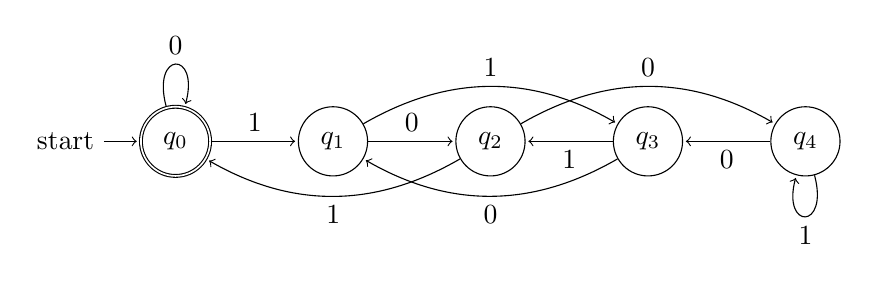
\begin{tikzpicture}[shorten >=1pt,node distance=2cm,on grid,auto]
            \node[state, accepting, initial] (q_0)   {$q_0$};
            \node[state] (q_1) [right=of q_0] {$q_1$};
            \node[state] (q_2) [right=of q_1] {$q_2$};
            \node[state] (q_3) [right=of q_2] {$q_3$};
            \node[state] (q_4) [right=of q_3] {$q_4$};
            \path[->]
                (q_0)
                    edge [loop above] node {0} (q_0)
                    edge node {1} (q_1)
                (q_1)
                    edge node {0} (q_2)
                    edge [bend right=-30] node {1} (q_3)
                (q_2)
                    edge [bend left] node {1} (q_0)
                    edge [bend right=-30] node {0} (q_4)
                (q_3)
                    edge node {1} (q_2)
                    edge [bend left] node {0} (q_1)
                (q_4)
                    edge node {0} (q_3)
                    edge [loop below] node {1} (q_4);
        \end{tikzpicture}
        \caption{DFA, \(A\), this is really beautiful, ya know?}
        \label{fig:multiple5}
    \end{figure}

    \textbf{Justification}
    \\

    Take a given binary number, \(x\). Since there are only two inputs to our
    state machine, \(x\) can either become \(x0\) or \(x1\). When a 0 comes
    into the state machine, it is the same as taking the binary number and
    multiplying it by two. When a 1 comes into the machine, it is the same as
    multipying by two and adding one.
    \\

    Using this knowledge, we can construct a transition table that tell us
    where to go:

    \begin{table}[ht]
        \centering
        \begin{tabular}{c || c | c | c | c | c}
            & \(x \mod 5 = 0\)
            & \(x \mod 5 = 1\)
            & \(x \mod 5 = 2\)
            & \(x \mod 5 = 3\)
            & \(x \mod 5 = 4\)
            \\
            \hline
            \(x0\) & 0 & 2 & 4 & 1 & 3 \\
            \(x1\) & 1 & 3 & 0 & 2 & 4 \\
        \end{tabular}
    \end{table}

    Therefore on state \(q_0\) or (\(x \mod 5 = 0\)), a transition line should
    go to state \(q_0\) for the input 0 and a line should go to state \(q_1\)
    for input 1. Continuing this gives us the Figure~\ref{fig:multiple5}.
\end{homeworkProblem}

\begin{homeworkProblem}
    Write part of \alg{Quick-Sort($list, start, end$)}

    \begin{algorithm}[]
        \begin{algorithmic}[1]
            \Function{Quick-Sort}{$list, start, end$}
                \If{$start \geq end$}
                    \State{} \Return{}
                \EndIf{}
                \State{} $mid \gets \Call{Partition}{list, start, end}$
                \State{} \Call{Quick-Sort}{$list, start, mid - 1$}
                \State{} \Call{Quick-Sort}{$list, mid + 1, end$}
            \EndFunction{}
        \end{algorithmic}
        \caption{Start of QuickSort}
    \end{algorithm}
\end{homeworkProblem}

\pagebreak

\begin{homeworkProblem}
    Suppose we would like to fit a straight line through the origin, i.e.,
    \(Y_i = \beta_1 x_i + e_i\) with \(i = 1, \ldots, n\), \(\E [e_i] = 0\),
    and \(\Var [e_i] = \sigma^2_e\) and \(\Cov[e_i, e_j] = 0, \forall i \neq
    j\).
    \\

    \part

    Find the least squares esimator for \(\hat{\beta_1}\) for the slope
    \(\beta_1\).
    \\

    \solution

    To find the least squares estimator, we should minimize our Residual Sum
    of Squares, RSS:

    \[
        \begin{split}
            RSS &= \sum_{i = 1}^{n} {(Y_i - \hat{Y_i})}^2
            \\
            &= \sum_{i = 1}^{n} {(Y_i - \hat{\beta_1} x_i)}^2
        \end{split}
    \]

    By taking the partial derivative in respect to \(\hat{\beta_1}\), we get:

    \[
        \pderiv{
            \hat{\beta_1}
        }{RSS}
        = -2 \sum_{i = 1}^{n} {x_i (Y_i - \hat{\beta_1} x_i)}
        = 0
    \]

    This gives us:

    \[
        \begin{split}
            \sum_{i = 1}^{n} {x_i (Y_i - \hat{\beta_1} x_i)}
            &= \sum_{i = 1}^{n} {x_i Y_i} - \sum_{i = 1}^{n} \hat{\beta_1} x_i^2
            \\
            &= \sum_{i = 1}^{n} {x_i Y_i} - \hat{\beta_1}\sum_{i = 1}^{n} x_i^2
        \end{split}
    \]

    Solving for \(\hat{\beta_1}\) gives the final estimator for \(\beta_1\):

    \[
        \begin{split}
            \hat{\beta_1}
            &= \frac{
                \sum {x_i Y_i}
            }{
                \sum x_i^2
            }
        \end{split}
    \]

    \pagebreak

    \part

    Calculate the bias and the variance for the estimated slope
    \(\hat{\beta_1}\).
    \\

    \solution

    For the bias, we need to calculate the expected value
    \(\E[\hat{\beta_1}]\):

    \[
        \begin{split}
            \E[\hat{\beta_1}]
            &= \E \left[ \frac{
                \sum {x_i Y_i}
            }{
                \sum x_i^2
            }\right]
            \\
            &= \frac{
                \sum {x_i \E[Y_i]}
            }{
                \sum x_i^2
            }
            \\
            &= \frac{
                \sum {x_i (\beta_1 x_i)}
            }{
                \sum x_i^2
            }
            \\
            &= \frac{
                \sum {x_i^2 \beta_1}
            }{
                \sum x_i^2
            }
            \\
            &= \beta_1 \frac{
                \sum {x_i^2 \beta_1}
            }{
                \sum x_i^2
            }
            \\
            &= \beta_1
        \end{split}
    \]

    Thus since our estimator's expected value is \(\beta_1\), we can conclude
    that the bias of our estimator is 0.
    \\

    For the variance:

    \[
        \begin{split}
            \Var[\hat{\beta_1}]
            &= \Var \left[ \frac{
                \sum {x_i Y_i}
            }{
                \sum x_i^2
            }\right]
            \\
            &=
            \frac{
                \sum {x_i^2}
            }{
                \sum x_i^2 \sum x_i^2
            } \Var[Y_i]
            \\
            &=
            \frac{
                \sum {x_i^2}
            }{
                \sum x_i^2 \sum x_i^2
            } \Var[Y_i]
            \\
            &=
            \frac{
                1
            }{
                \sum x_i^2
            } \Var[Y_i]
            \\
            &=
            \frac{
                1
            }{
                \sum x_i^2
            } \sigma^2
            \\
            &=
            \frac{
                \sigma^2
            }{
                \sum x_i^2
            }
        \end{split}
    \]

\end{homeworkProblem}

\pagebreak

\begin{homeworkProblem}
    Prove a polynomial of degree \(k\), \(a_kn^k + a_{k - 1}n^{k - 1} + \hdots
    + a_1n^1 + a_0n^0\) is a member of \(\Theta(n^k)\) where \(a_k \hdots a_0\)
    are nonnegative constants.

    \begin{proof}
        To prove that \(a_kn^k + a_{k - 1}n^{k - 1} + \hdots + a_1n^1 +
        a_0n^0\), we must show the following:

        \[
            \exists c_1 \exists c_2 \forall n \geq n_0,\ {c_1 \cdot g(n) \leq
            f(n) \leq c_2 \cdot g(n)}
        \]

        For the first inequality, it is easy to see that it holds because no
        matter what the constants are, \(n^k \leq a_kn^k + a_{k - 1}n^{k - 1} +
        \hdots + a_1n^1 + a_0n^0\) even if \(c_1 = 1\) and \(n_0 = 1\).  This
        is because \(n^k \leq c_1 \cdot a_kn^k\) for any nonnegative constant,
        \(c_1\) and \(a_k\).
        \\

        Taking the second inequality, we prove it in the following way.
        By summation, \(\sum\limits_{i=0}^k a_i\) will give us a new constant,
        \(A\). By taking this value of \(A\), we can then do the following:

        \[
            \begin{split}
                a_kn^k + a_{k - 1}n^{k - 1} + \hdots + a_1n^1 + a_0n^0 &=
                \\
                &\leq (a_k + a_{k - 1} \hdots a_1 + a_0) \cdot n^k
                \\
                &= A \cdot n^k
                \\
                &\leq c_2 \cdot n^k
            \end{split}
        \]

        where \(n_0 = 1\) and \(c_2 = A\). \(c_2\) is just a constant. Thus the
        proof is complete.
    \end{proof}
\end{homeworkProblem}

\pagebreak

%
% Non sequential homework problems
%

% Jump to problem 18
\begin{homeworkProblem}[18]
    Evaluate \(\sum_{k=1}^{5} k^2\) and \(\sum_{k=1}^{5} (k - 1)^2\).
\end{homeworkProblem}

% Continue counting to 19
\begin{homeworkProblem}
    Find the derivative of \(f(x) = x^4 + 3x^2 - 2\)
\end{homeworkProblem}

% Go back to where we left off
\begin{homeworkProblem}[6]
    Evaluate the integrals
    \(\int_0^1 (1 - x^2) \dx\)
    and
    \(\int_1^{\infty} \frac{1}{x^2} \dx\).
\end{homeworkProblem}

\end{document}
